%%%%%%%%%%%%%%%%%%%%%%%%%%%%%%%%%%%%%%%%%%%%%%%%%%%%%%%%%%%%%
\begin{frame} [plain]
    \frametitle{}
    \Background[1] 
    \begin{center}
    {\huge 第7讲:压缩态}
    \end{center}  
    \addtocounter{framenumber}{-1}   
\end{frame}
%%%%%%%%%%%%%%%%%%%%%%%%%%%%%%%%%%%%%%%%%%%%%%%%%%%%%%%%%%%% 

\section{1. 压缩态基本概念}

\begin{frame}
    \frametitle{}
    \begin{tcolorbox3}[前情回顾]
     \begin{itemize}
                \item 真空态是最小不确定度乘积态
                \item 相干态也是小不确定度乘积态
                \[ \Delta X_1 \Delta X_2 =\dfrac{1}{4}, \, \Delta X_1 = \Delta X_2 = \frac{1}{2} \] 
         \end{itemize}
    \end{tcolorbox3}
\end{frame}

\begin{frame}
 \frametitle{}
      \begin{center}
           \begin{tcolorbox2}[0.86]{压缩态的定义:}
            某正交分量的涨落被压缩的最小不确定度乘积态($\Delta X_i < \dfrac{1}{2}$)
            \[ \Delta X_1 \Delta X_2 =\dfrac{1}{4}, \, \Delta X_1 \not = \Delta X_2  \] 
            \centering
            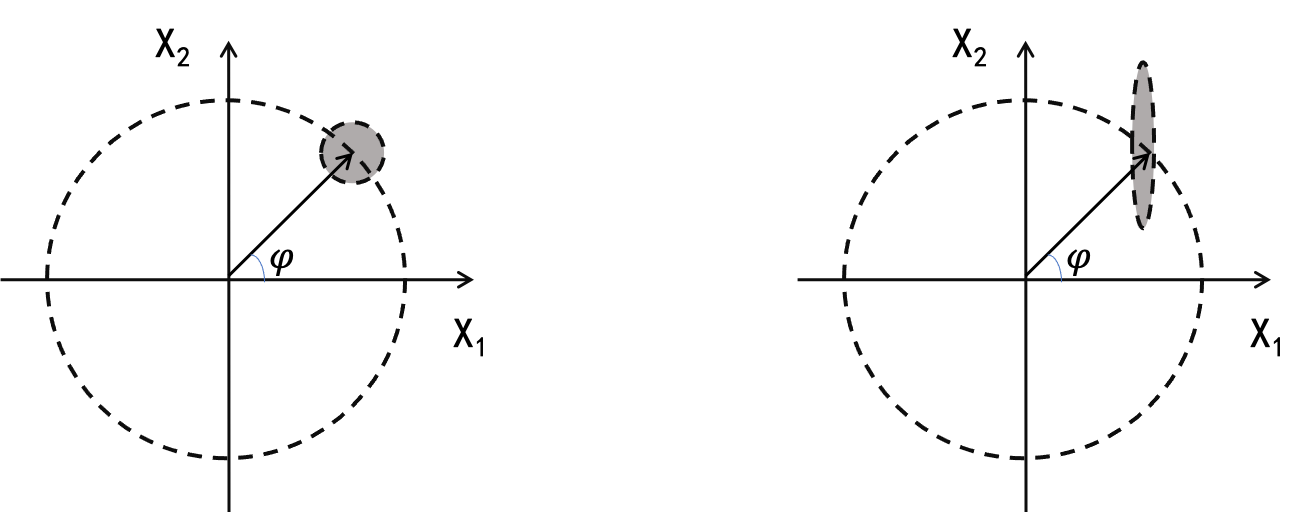
\includegraphics[width=0.66\textwidth]{figs/6.png}
          \end{tcolorbox2}  
      \end{center} 
\end{frame}

\begin{frame}
 \frametitle{}
 发展与影响:
 \begin{itemize}
     \item  1970年 D. Stoler[1], 提出压缩相干态概念。
     \item  1980年 压缩态得以实现并发展到最高可压缩80\%
     \item  随后逐渐应用到各种精密测量和量子通讯, 并在引力波测量中大显身手 
     \item 基此衍生的纠缠光子双技术,也已成为量子加密和量子计算的重要基础。
 \end{itemize}
 ~~ \\ {\vspace*{2.8em}}
 (1) D. ~Stoler, Phys. Rev.  A ~ 131, 2766(1970)    
\end{frame}

\begin{frame}
 \frametitle{谐振子基态的压缩}
 谐振子哈密顿
 \[  H= \frac{p^2}{2m} +\frac{1}{2}m \omega^2 q^2\]
 作如下变化, 试求解谐振子 
 \[  H= \frac{p^2}{2m} +\frac{1}{2}m \omega^2 q^2 +c \]
 \[  H= \frac{p^2}{2m} +\frac{1}{2}m \omega^2 q^2 +cq\]
 \[  H= \frac{p^2}{2m} +\frac{1}{2}m \omega^2 q^2 +cq^2\]
 \end{frame}
 
 \begin{frame}
       \frametitle{}     
  \解 (1) 
    \[\begin{aligned}
    H &= \frac{p^2}{2m} +\frac{1}{2}m \omega^2 q^2 +c \\  
    H-c &= \frac{p^2}{2m} +\frac{1}{2}m \omega^2 q^2  \\ 
    H' &= \frac{p^2}{2m} +\frac{1}{2}m \omega^2 q^2  \\   
    \end{aligned} \]    
*只是能级发生的整体的平衡, 不影响谐振子基态波包的形态   
\end{frame}

\begin{frame}
 \frametitle{}
 (2) 

   \[\begin{aligned}
    H &= \frac{p^2}{2m} +\frac{1}{2}m \omega^2 q^2 +cq \\ 
    H-c_2 &= \frac{p^2}{2m} +\frac{1}{2}m \omega^2 (q+c_1)^2  \\ 
    H' &= \frac{p^2}{2m} +\frac{1}{2}m \omega^2 (q')^2  \\ 
   \end{aligned} \]    
  
 * 能级和位置都发生整体平衡, 不影响谐振子基态波包的形态
\end{frame}

\begin{frame}
 \frametitle{}
  (3)  
    \[\begin{aligned}
        H &= \frac{p^2}{2m} +\frac{1}{2}m \omega^2 q^2 +cq^2 \\ 
        H &= \hbar \omega (a^\dagger a +\frac{1}{2}) +cq^2  \\ 
        H  &= \hbar \omega (a^\dagger a +\frac{1}{2}) +c \frac{\hbar}{2m \omega} (a^2 + a^{\dagger 2} + 2 a^\dagger a +1 ) \\ 
        H-c_2 &= c_0\hbar \omega (a^\dagger a +\frac{1}{2}) +c_1 (a^2 + a^{\dagger 2})  \\ 
        H' &= c_0\hbar \omega (a^\dagger a +\frac{1}{2}) +c_1 (a^2 + a^{\dagger 2})  \\ 
    \end{aligned} \]    
    这是一个收缩的势阱, 增加的$a^2$ 和 $a^{\dagger 2}$ 称之为“双光子项”, 涉及到光子的二次产生和湮灭过程, 导致谐振子基态波包的形态发生变化(被压缩)
\end{frame}

\begin{frame}
 \frametitle{}
 (4)  
 考虑如下哈密顿 
 \[\begin{aligned}
     H &= \frac{(p/\xi)^2}{2m} +\frac{1}{2}m \omega^2 (\xi q)^2  \\ 
 \end{aligned} \]    
 它直接对正则位置和动量进行了伸缩操作, 因此求解过程与原来的完全一样. 基态还是最小不确定度乘积态
 \[ \Delta X_1 \Delta X_2 =\dfrac{1}{4}\] 
 但涨落却变为 
 \[ \Delta X_1  = \frac{1}{2 \xi^2}, \, \Delta X_2  = \frac{\xi^2}{2}\]  
 $\left|\xi\right|>1$, 实现对 $X_1 $ 的压缩. $\left|\xi\right|<1$, 则实现对 $X_2 $ 的压缩. 

 
\end{frame}



\section{2. 压缩算符}

\begin{frame}
 \frametitle{}
 \begin{center}
    \begin{tcolorbox2}[0.86]{压缩算符的定义:}
    \[ S(\xi) = e^{\frac{1}{2}[\xi^* a^2 - \xi (a^{\dagger}) ^2]}\]
    其中压缩参量$\xi= r e^{i\theta}$, r 称为压缩幅,描述压缩的大小; $\theta$ 称为压缩角,描述压缩的方向. \\
    明显:  
    \[ S(\xi)^\dagger = e^{-\frac{1}{2}[\xi^* a^2 - \xi a^{\dagger 2}]}\]
   \end{tcolorbox2}  
\end{center}    
\end{frame}

\begin{frame}
 \frametitle{}
 \例 [1. 试证明压缩态算符有如下特点]{
    \begin{enumerate}
        \item 压缩算符不是厄密算符
        \item 压缩算符是幺正算符
    \end{enumerate}
    } 
    \证 ~ (1) 由定义,有 $S \not = S^\dagger$, 因此 压缩算符不是厄密算符 \\ 
    \证 ~(2) 计算
    \[\begin{aligned}
        S S^\dagger = S^\dagger S = e^{-\frac{1}{2}[\xi^* a^2 - \xi (a^{\dagger}) ^2]} e^{\frac{1}{2}[\xi^* a^2 - \xi (a^{\dagger}) ^2]} =e^0 =1
    \end{aligned} \]
     因此,  $S^\dagger = S^{-1} $,  压缩算符是幺正算符
\end{frame}

\begin{frame}
 \frametitle{压缩态}
  \begin{enumerate}
      \item 压缩真空态是一种压缩态,由压缩算符作用于真空态产生
     \[ \rs{\xi } = S(\xi) \rs{0 }  \]
      \item 压缩相干态也是一种压缩态,由压缩算符作用于相干态产生
    \[\begin{aligned}
          \rs{\alpha,\xi } &= S(\xi) \rs{\alpha } \\ 
          &=  S(\xi) D(\alpha) \rs{0} \\
          & \not = D(\alpha)S(\xi) \rs{0} 
    \end{aligned} \]  
  \end{enumerate}
  显然,压缩真空态只是相图在原点的特殊压缩态 $ \rs{0,\xi } $, 若不考虑对哪个态的压缩, 压缩态可记为 $\rs{\xi }$
\end{frame}

\begin{frame}
    \frametitle{}
    \例 [2. 试证明产生湮灭算符对压缩态的期望值为]{
    \[ \langle\xi|a| \xi\rangle=\alpha \cosh r- \alpha^{*}  e^{i\theta}\sinh r , \quad \left\langle\xi\left|a^{\dagger}\right| \xi\right\rangle=\alpha^{*} \cosh r -\alpha  e^{-i\theta}\sinh r \]
    } 
    \证 ~有算符的$Baker-Campbell-Hausdorff$ 公式
    \[ e^A B e^{-A} = B+ [A,B] + \frac{1}{2!}[A,[A,B]] + \cdots \]
    先做算符计算
    \[\begin{aligned}
        S^\dagger a S &= e^{-\frac{1}{2}[\xi^* a^2 - \xi (a^{\dagger}) ^2]} a  e^{\frac{1}{2}[\xi^* a^2 - \xi (a^{\dagger}) ^2]} \\ 
        &=  a -\xi a^\dagger + \frac{1}{2!} \left|\xi\right|^2 a - \frac{1}{3!} \xi \left|\xi\right|^2 a^\dagger + \cdots \\  
        &=  a \left( 1 + \frac{\left|\xi\right|^2 }{2!} + \frac{\left|\xi\right|^4}{4!} + \cdots\right) - a^\dagger \left(  \xi  + \frac{\xi \left|\xi\right|^2}{3!} +   \frac{\xi \left|\xi\right|^4}{5!} + \cdots \right)\\ 
        &= a \cosh r- a^{\dagger}  e^{i\theta}\sinh r 
  \end{aligned} \]      
   \end{frame}

   \begin{frame}
    \frametitle{}
    再计算期望值:
    \[\begin{aligned}
        \langle\xi |a| \xi\rangle &= \lcr {\alpha} {S^\dagger a S}{\alpha}  \\ 
        &= \lcr {\alpha} { a \cosh r- a^{\dagger}  e^{i\theta}\sinh r}{\alpha}  \\ 
        &= \lcr {\alpha} {\alpha \cosh r- \alpha^{*}  e^{i\theta}\sinh r }{\alpha}  \\ 
        &= \alpha \cosh r- \alpha^{*}  e^{i\theta}\sinh r 
  \end{aligned} \] 
  同理, 有 
  \[  S^\dagger a S = a^{\dagger} \cosh r -a  e^{-i\theta}\sinh r \]
  \[ \left\langle\xi\left|a^{\dagger}\right| \xi\right\rangle=\alpha^{*} \cosh r -\alpha  e^{-i\theta}\sinh r\]
   \end{frame}


   \begin{frame}
    \frametitle{}
    记双曲函数为: \[ \begin{gathered}
        \mu=\cosh r=\frac{e^{r}+e^{-r}}{2} \\
        \nu=e^{i \theta} \sinh r=\frac{e^{r}-e^{-r}}{2}
        \end{gathered} \]
    有:
    \[\begin{aligned}
        S^\dagger a S &= \mu a - \nu a^{\dagger}  \\ 
        S^{\dagger} a^{\dagger} S &=\mu a^{\dagger}-\nu^{*} a \\
        S a S^{\dagger} &=\mu a+\nu a^{\dagger}  = a(\xi) \\
        S a^{\dagger} S^{\dagger} &=\mu a^{\dagger}+\nu^{*} a   = a^{\dagger} (\xi) 
        \end{aligned} \]    
   \end{frame}

   \begin{frame}
    \frametitle{}
    对压缩态有如下均值: 
       \[ \begin{aligned}
           \langle a\rangle &=\mu\alpha - \nu \alpha^{*}  = \alpha_{-}\\
           \left\langle a^{\dagger}\right\rangle &= \mu \alpha^{\dagger}-\nu^{*} \alpha = \alpha_{-} ^*\\
           \left\langle a^{2}\right\rangle &=\alpha^{2} \mu^{2}+\alpha^{* 2} \nu^{2}-2|\alpha|^{2} \mu \nu-\mu \nu =  \alpha_\xi ^{2}- e^{i\theta} \sinh r \cosh r \\
           \left\langle a^{\dagger 2} \right\rangle &= \alpha_\xi ^{*2}- e^{-i\theta} \sinh r \cosh r  \\ 
           \left\langle a^{\dagger} a\right\rangle &=|\alpha|^{2}\left(\mu^{2}+|\nu|^{2}\right)-\alpha^{* 2} \mu \nu-\alpha^{2} \mu \nu^{*}+|\nu|^{2}
           \end{aligned}\]
   \end{frame}


   \begin{frame}
    \frametitle{}
    \例 [3.  试证明压缩态是算符$ S a S^\dagger $的本征态 ]{
        ~\\ 
    \[ \boxed{S a S^\dagger \rs{\xi } = \alpha \rs{\xi } }\]}
    \证~  
    \[\begin{aligned}
        S a S^\dagger \rs{\xi } &= S a S^\dagger S \rs{\alpha } \\ 
        &= S a \rs{\alpha } \\ 
        &= S \alpha \rs{\alpha } \\ 
        &= \alpha  S \rs{\alpha } \\ 
        &= \alpha   \rs{\xi }  \\ 
        a(\xi) \rs{\xi } &= \alpha   \rs{\xi }
    \end{aligned} \]
    上式中, 令 \[\hat{a}(\xi)=  \hat{S} \hat{a} \hat{S}^\dagger = \mu \hat{a}+\nu \hat{a}^{\dagger} , \qquad  \hat{a}^\dagger (\xi)=  \hat{S} \hat{a}^\dagger \hat{S}^\dagger =\mu \hat{a}^{\dagger}+\nu^{*} \hat{a} \]
   \end{frame}

   \begin{frame}
    \frametitle{}
         先压缩还是先平移? (我们定义左边的先有!)
         \[\begin{aligned}
            \rs{\alpha,\xi } &= S(\xi) \rs{\alpha } \\ 
            &=  S(\xi) D(\alpha) \rs{0} \\
            \rs{\xi, \alpha} &= D(\alpha) \rs{\xi } \\ 
            &=   D(\alpha) S(\xi)\rs{0} \\
        \end{aligned} \]
        交换次序相当于幺正变换 \\ 
        \证~ 
        \[\begin{aligned}
            S(\xi) D(\alpha) & = S(\xi) D(\alpha)S^\dagger (\xi) S(\xi) \\ 
            S(\xi) D(\alpha) & =  D(\alpha_{+}) S(\xi) \\ 
            \to  \alpha_{+ } &= \mu\alpha  +  \nu \alpha^{*} \\ 
            &= \alpha \cosh r + \alpha^{*} e^{i \theta} \sinh r
        \end{aligned} \]
    \end{frame}


    \begin{frame}
     \frametitle{} 

        \[\begin{aligned}
            \rs{\alpha,\xi } & = S(\xi) D(\alpha) \rs{0}  \\ 
            &= S(\xi) D(\alpha)S^\dagger (\xi) S(\xi) \rs{0} \\ 
            &= D(\alpha_{+}) S(\xi) \rs{0} \\ 
            &= D(\alpha_{+}) \rs{\xi} \\ 
            &= \rs{\xi, \alpha_{+}} 
        \end{aligned} \]
        同理: 
        \[\begin{aligned}
            \rs{\xi, \alpha }& = \rs{\alpha_{-},\xi} \\ 
            \alpha_{- } &= \mu\alpha  -  \nu \alpha^{*} \\ 
            &= \alpha \cosh r - \alpha^{*} e^{i \theta} \sinh r
        \end{aligned} \]
    \end{frame}
    
    \begin{frame}
          \frametitle{}
          
    压缩相干态是如下本征方程的本征矢: 
    \[\begin{aligned}
        a(\xi) \rs{\alpha, \xi} &= S(\xi) a S ^\dagger (\xi) \rs{\alpha, \xi}  \\ 
        &= S(\xi) a S ^\dagger (\xi) \rs{\xi, \alpha_{+}}  \\ 
        &= S (\xi)  a  \rs{0, \alpha_{+}} \\ 
        &= S (\xi) \alpha_{+}  \rs{0, \alpha_{+}} \\ 
        &= \alpha_{+} S (\xi)  \rs{0, \alpha_{+}} \\ 
        &= \alpha_{+}  \rs{\xi, \alpha_{+}} \\ 
        &= \alpha_{+}  \rs{\alpha, \xi}  
    \end{aligned} \]

    \[  \boxed{a(\xi) \rs{\alpha, \xi}= \alpha_{+}  \rs{\alpha, \xi}}\]
   
   \end{frame}

\section{3. 压缩态的场性质}

\begin{frame}
 \frametitle{}
 \例 [4.试计算压缩态场的正交分量算符的量子涨落 ]{
    \[ \Delta X_1 \Delta X_2 =\dfrac{1}{4}, \qquad  \Delta X_1 = \frac{1}{2} e^{-r} < \frac{1}{2}, \, \Delta X_2 = \frac{1}{2} e^r > \frac{1}{2}, (\text{for} \quad r>0)\]}
    \解~  
    \[\begin{aligned}
        \left\langle X_1 \right\rangle &= \lcr {\xi} {X_1} {\xi}\\
        &= \frac{1}{2}\lcr {\alpha} {S^\dagger(a+ a^{\dagger})S } {\alpha}\\
        &= \frac{1}{2}(\lcr {\alpha} {S^\dagger a S + S^\dagger a^{\dagger}S } {\alpha} )  \\ 
        &= \frac{1}{2}(\left\langle a \right\rangle + \left\langle a^\dagger \right\rangle)  \\ 
        &= \frac{1}{2}( \alpha \cosh r- \alpha^{*}  e^{i\theta}\sinh r + \alpha^{*} \cosh r -\alpha  e^{-i\theta}\sinh r ) \\ 
        &= \frac{1}{2} \mathrm{e}^{-r} (\alpha + \alpha^*)  
    \end{aligned} \]
\end{frame}

\begin{frame}
 \frametitle{}
 \[\begin{aligned}
    \left\langle X_1 ^2 \right\rangle &= \lcr {\xi} {X_1 ^2} {\xi}\\
    &= \frac{1}{4}\lcr {\xi} {(a+ a^{\dagger})^2 } {\xi}\\
    &= \frac{1}{4}(\lcr {\xi} { a^2 + a^{\dagger 2 }  + a a^{\dagger} + a^{\dagger} a } {\xi} )  \\ 
    &= \frac{1}{4}(\lcr {\xi} { a^2 + a^{\dagger 2 }  + 2 a^{\dagger} a +1 } {\xi} )  \\ 
    &= \frac{1}{4}( \left\langle a^2 \right\rangle + \left\langle a^{\dagger 2 } \right\rangle + \left\langle 2 a^{\dagger} a \right\rangle ) + \frac{1}{4} e^{-2r}    \\ 
    &= \frac{1}{4} \mathrm{e}^{-2r} (\alpha + \alpha^*)^2 +  \frac{1}{4} e^{-2r} 
\end{aligned} \]
\end{frame}

\begin{frame}
    \frametitle{}
    \[\begin{aligned}
       \Delta X_1 &= \sqrt{ \left\langle X_1 ^2 \right\rangle - \left\langle X_1 \right\rangle ^2 } \\ 
       &=\frac{1}{2} e^{-r} < \frac{1}{2} 
   \end{aligned} \]     
   同理, 有: 
   \[\begin{aligned}
    \left\langle X_2 \right\rangle &= \frac{1}{2i} \mathrm{e}^{r} (\alpha - \alpha^*) \\ 
    \Delta X_2 &= \frac{1}{2} e^{r}  > \frac{1}{2}
\end{aligned} \]  
\end{frame}

\begin{frame}
      \frametitle{}
  对于压缩真空态$\alpha=0$, 
  \[\begin{aligned}
    \left\langle X_1 \right\rangle=\left\langle X_2 \right\rangle &= 0 \\ 
    \left\langle X_1 ^2 \right\rangle=\left\langle X_2 ^2 \right\rangle & \not = 0 \\ 
    \Delta X_1 \Delta X_2 = \frac{1}{2} e^{-r} \frac{1}{2} e^{r} &= \dfrac{1}{4}
\end{aligned} \]  

对于压缩相干态$\alpha \not = 0$, 
\[\begin{aligned}
  \left\langle X_1 \right\rangle=\left\langle X_2 \right\rangle & \not = 0 \\ 
  \left\langle X_1 ^2 \right\rangle=\left\langle X_2 ^2 \right\rangle & \not = 0 \\ 
  \Delta X_1 \Delta X_2 = \frac{1}{2} e^{-r} \frac{1}{2} e^{r} &= \dfrac{1}{4}
\end{aligned} \] 

* 压缩态的一个正交分量被压缩,而另一个被等比例放大. 依然是最小不确定度乘积态!
\end{frame}


\begin{frame}  
    \frametitle{坐标轴的旋转}
    正交分量算符的旋转:    
    $$\left\{\begin{matrix}
        Y_1=X_1\cos\theta /2 +X_2\sin\theta /2\\
        Y_2=-X_1\sin\theta /2 +X_2\cos\theta /2
    \end{matrix}\right.$$
    $$\begin{bmatrix}
        Y_1 \\
        Y_2
    \end{bmatrix}
    =
    \begin{bmatrix}
        \cos\theta /2 & \sin\theta /2\\
        -\sin\theta /2 & \cos\theta /2
    \end{bmatrix}
    \begin{bmatrix}
        X_1 \\
        X_2
    \end{bmatrix}$$
    $$ R_{\theta /2}=
    \begin{bmatrix}
        \cos\theta  /2 &\sin\theta /2\\
        -\sin\theta /2 &\cos\theta /2
    \end{bmatrix} ,\qquad
    R_{\theta  /2} ^{\dagger}=
    \begin{bmatrix}
        \cos\theta /2 & -\sin\theta /2\\
        \sin\theta /2 &\cos\theta /2
    \end{bmatrix} $$
    代入 $X_1, X_2$, 得到用产生湮灭算符表述的形式: 
    $$\left\{\begin{matrix}
        Y_1=\frac{1}{2}(a e^{-i \theta /2 }+a^\dagger e^{i \theta /2 })\\
        Y_2=\frac{1}{2i}(a e^{-i \theta /2 }-a^\dagger e^{i \theta /2 })
    \end{matrix}\right.$$
   \[ \]
\end{frame}

\begin{frame}
 \例 [5.  对压缩态,求旋转正交分量算符的的均值和涨落]{
 }
  \解~ 先计算如下均值: 
  \[ \begin{aligned}
    \lcr{\xi}{Y_1 }{\xi} &= \frac{1}{2} \mathrm{e}^{-r} (\alpha \mathrm{e}^{-i\frac{\theta}{2}}+ \alpha^* \mathrm{e}^{i\frac{\theta}{2}})   \\ 
    \lcr{\xi}{Y_2 }{\xi} &= \frac{1}{2i} \mathrm{e}^{-r} (\alpha \mathrm{e}^{-i\frac{\theta}{2}}- \alpha^* \mathrm{e}^{i\frac{\theta}{2}})   \\ 
    \lcr{\xi}{Y_1 ^2 }{\xi} &=  \frac{1}{4} \mathrm{e}^{-2r} (\alpha \mathrm{e}^{-i\frac{\theta}{2}}+ \alpha^* \mathrm{e}^{i\frac{\theta}{2}})^2 +  \frac{1}{4} e^{-2r}  \\ 
    \lcr{\xi}{Y_2 ^2 }{\xi} &= -\frac{1}{4} \mathrm{e}^{-2r} (\alpha \mathrm{e}^{-i\frac{\theta}{2}}- \alpha^* \mathrm{e}^{i\frac{\theta}{2}})^2  +  \frac{1}{4} e^{ 2r}  \\ 
\end{aligned}\]

\end{frame}

\begin{frame}
  再计算涨落:  \\
  \[\begin{aligned}
    \Delta Y_1 &= \sqrt{ \left\langle Y_1 ^2 \right\rangle - \left\langle Y_1 \right\rangle ^2 } \\ 
    &=\frac{1}{2} e^{-r}  \\ 
 \Delta Y_2 &= \frac{1}{2} e^{r}  \\ 
\end{aligned} \]  
 不确定度关系: 
 \[  \Delta X_1 \Delta X_2 = \frac{1}{2} e^{-r} \frac{1}{2} e^{r} = \dfrac{1}{4} \]

 \begin{itemize}
     \item $ r>0, \Delta Y_1 < \frac{1}{2} $, 压缩振幅 
     \item $ r<0, \Delta Y_2 < \frac{1}{2} $, 压缩相位
 \end{itemize}


\end{frame}

\begin{frame}
 \frametitle{}
 压缩态相图
   \begin{center}
        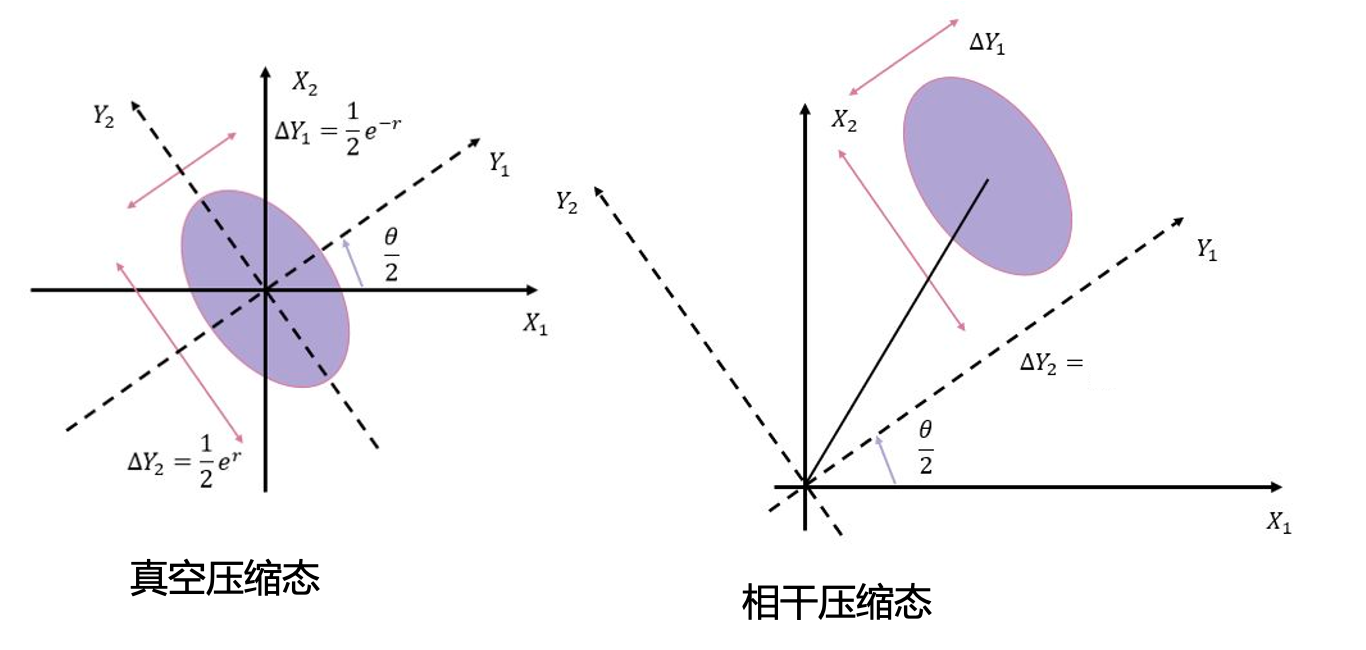
\includegraphics[width=1.0\textwidth]{figs/2022-05-02-13-13-46.png}
   \end{center}   
\end{frame}

\begin{frame}
    \frametitle{}
    压缩态相图
      \begin{center}
           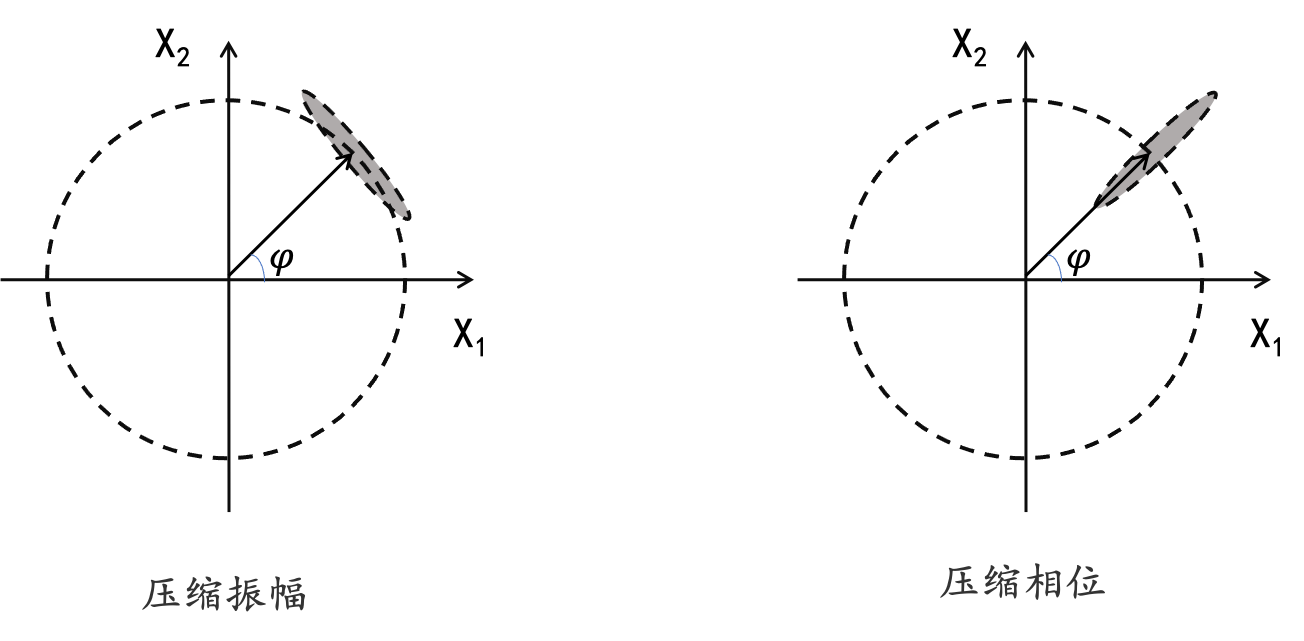
\includegraphics[width=1.0\textwidth]{figs/9.png}
      \end{center}   
   \end{frame}

\begin{frame}
 \frametitle{}
      光场的量子涨落:
      \[ \overline{ (\Delta \mathbf{E}(\mathbf{r},t))^2} = \frac{1}{L^3} (\frac{2\hbar \omega}{\epsilon_0}) [ \overline{ (\Delta X_1)^2} \sin ^2 (\omega t - \mathbf{k}\cdot \mathbf{r}) + \overline{ (\Delta X_2)^2} \cos ^2 (\omega t - \mathbf{k}\cdot \mathbf{r}) ]\]
\end{frame}

   \begin{frame}
    \frametitle{}
    压缩态波形图
      \begin{center}
           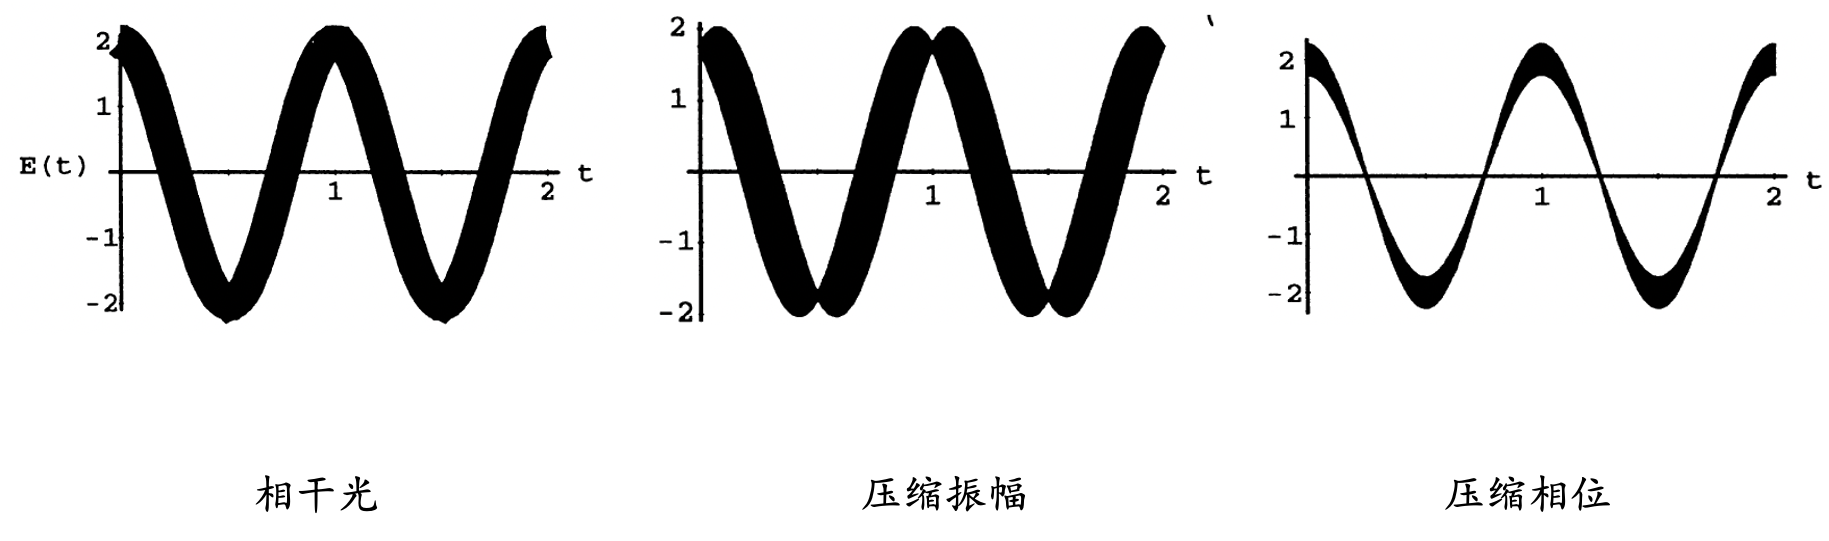
\includegraphics[width=1.0\textwidth]{figs/12.png}
      \end{center}   
   \end{frame}

\begin{frame}
    \例 [6.  求压缩态光子数的均值和涨落]{
    }
     \解~ 先计算如下均值: 
      \[ \begin{aligned}
        \overline{n} & = \left\langle a^{\dagger} a\right\rangle  \\ 
        &= \lcr{\xi} {a^{\dagger} a} {\xi} \\ 
        &= \lcr{\xi} {|\alpha|^{2}\left(\mu^{2}+|\nu|^{2}\right)-\alpha^{* 2} \mu \nu-\alpha^{2} \mu \nu^{*}+|\nu|^{2}} {\xi} \\ 
        &= (\mu \alpha^* _{+} - \nu^* \alpha _{+})(\mu \alpha _{+} - \nu \alpha ^* _{+}) + \left| \nu ^2 \right| \\ 
        &= \left|\alpha^2\right| + \left| \nu ^2 \right| \\ 
        &= \left|\alpha^2\right| + \sinh ^2 (r)
       \end{aligned}\]  
       如果是真空压缩态, $\alpha=0 $, 光子数均值为 $\sinh ^2 (r)$  
   \end{frame}

   \begin{frame}
    \frametitle{}
    \[ \begin{aligned}
        \overline{n^2} & = \left\langle (a^{\dagger} a)^2\right\rangle  \\ 
        &= \lcr{\xi} {a^{\dagger} a a^{\dagger} a} {\xi} \\ 
        &= \lcr{\xi} {a^{\dagger} (a a^{\dagger}) a} {\xi} \\ 
        &= \lcr{\xi} {a^{\dagger} (a^{\dagger} a +1) a} {\xi} \\ 
        &= \lcr{\xi} {a^{\dagger 2 }  a ^2 + a^{\dagger }a} {\xi} \\ 
        &= \lcr{\xi} {a^{\dagger 2 }  a ^2 } {\xi} +  \lcr{\xi} { a^{\dagger} a} {\xi} \\ 
        &= \overline{a^{\dagger 2 }  a ^2 } + \overline{n}
       \end{aligned}\] 
       式中,双光子项为 
       \[  \overline{a^{\dagger 2 }  a ^2 } = \left| \alpha ^4 \right| + \mu ^2 \left|\nu^2\right| - \mu (\alpha^2 \nu^* +cc) + 4 \left|\alpha^2 \right| \left|\nu^2\right| + 2 \left|\nu ^4\right|\] 
   \end{frame}

   \begin{frame}
    \frametitle{}
        粒子数涨落: 
    \[\begin{aligned}
             \Delta n & =\sqrt{ \overline{n^2} - (\overline{n})^2 } \\ 
             &= \sqrt{ \overline{a^{\dagger 2 }  a ^2 } + \overline{n} - (\overline{n})^2 }
    \end{aligned} \]
        占据数分布: 
      \begin{center}
           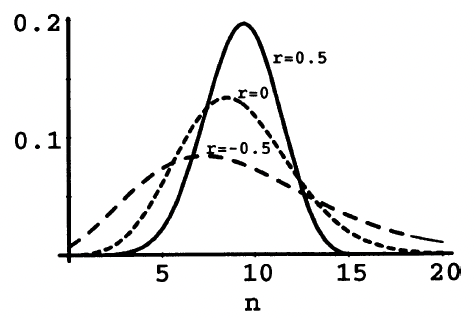
\includegraphics[width=0.5\textwidth]{figs/2022-05-03-23-54-35.png}
      \end{center}

   \end{frame}

   \begin{frame}
    \frametitle{压缩态随时间的演化}
    撤去外加势场后,相干态随着时间演化规律是,波包位置谐振但形状不变。下面考虑在撤去外加势场后,压缩态波包随时间的演化 \\   
    \例 [7.  求压缩态随时间的演化规律]{
    }
    \解~ 增加时间演化因子, 场的正交分量为: 
    $$\left\{\begin{matrix}
        Y_1=\dfrac{1}{2}(a e^{-i (\omega t + \theta /2) }+a^\dagger e^{i (\omega t + \theta /2) })\\ 
        Y_2=\dfrac{1}{2i}(a e^{-i (\omega t + \theta /2) }-a^\dagger e^{i (\omega t + \theta /2) })
    \end{matrix}\right.$$
   \end{frame}

   \begin{frame}
    \frametitle{}
     对于压缩态,求均值, 可得: 
    \[ 
        \begin{aligned}
            &\left\langle Y_{1}(t)\right\rangle=\frac{1}{2} e^{-r}\left(\alpha e^{-i\left(\omega t+\frac{\theta}{2}\right)}+\alpha^{*} e^{i\left(\omega t+\frac{\theta}{2}\right)}\right) \\
            &\left\langle Y_{2}(t)\right\rangle=\frac{1}{2 i} e^{r}\left(\alpha e^{-i\left(\omega t+\frac{\theta}{2}\right)}-\alpha^{*} e^{i\left(\omega t+\frac{\theta}{2}\right)}\right) \\
            &\Delta Y_{1}(t)=\frac{1}{2} e^{-r} \\
            &\Delta Y_{2}(t)=\frac{1}{2} e^{r}
            \end{aligned} \]
    均值随时间谐振,即波包整体做简谐运动;场正交涨落值不变,波包形状不变  \\ 
    (见动画)
   \end{frame}

   \section{4. 压缩态的产生}

   \begin{frame}
    \frametitle{压缩态的产生}
  理论上,就是要基于非线性效应,构造含双光子过程的系统, 具有如下压缩算符. 
  \[ S(\xi) = e^{\frac{1}{2}[\xi^* a^2 - \xi (a^{\dagger}) ^2]}\]

  \begin{itemize}
      \item  参量放大下转换
      \item  铁电原子系综三阶非线性效应 ~~ 四波混频
      \item  光纤的三阶非线性效应
      \item  二次谐波
      \item 共振荧光
  \end{itemize}

  \end{frame}
  
  \begin{frame}
        \frametitle{参量下转换}
  非线性介质具有多光子过程: \\ 
  介质中, 电位移矢量与场强和极化矢量有如下关系:
  \[ \mathbf{D}=\epsilon_0 \mathbf{E} + \mathbf{P}  \]
  通常, 可以认为 $\mathbf{P}$ 对 $\mathbf{E}$ 是线性的. 
  \[\mathbf{P}(\omega)= \epsilon_0 \chi(\omega) \mathbf{E}(\omega) \]
  实际上, 它的Taylor展开如下: (线性只是其一阶近似).
  \[ P_{i}=\varepsilon_{0}\left[\chi_{i j}^{(1)} E_{j}+\chi_{i j k}^{(2)} E_{j} E_{k}+\chi_{i j k l}^{(3)} E_{j} E_{k} E_{l}+\cdots\right] \]
  考虑二阶项, 对应材料吸收一种频率的光子,产生倍频成分新光子. 称为非线性介质的参量下转换过程. 
\end{frame}

\begin{frame}
 \frametitle{}
        \begin{center}
             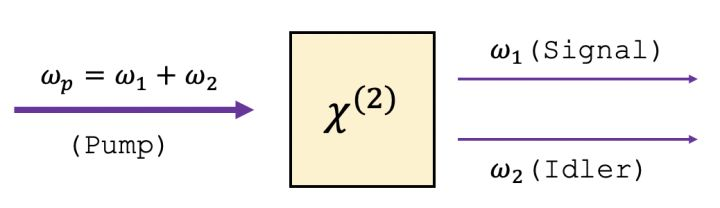
\includegraphics[width=0.7\textwidth]{figs/2022-05-02-20-00-04.png}
        \end{center}
        考虑简并参量放大 (OPA) $\omega_s = \omega_i = \omega = \frac{1}{2} \omega_p$, 这个过程的哈密顿 可写成: 
    \[ 
        \begin{aligned}
            H_{nl} & = \gamma  \Phi\left(k_{p} ; k_{1}, k_{2}\right) a_{k_{p}} ^ \dagger  a_{k_{1}} a_{k_{2}} - \gamma  \Phi\left(k_{p} ; k_{1}, k_{2}\right) a_{k_{p}} a_{k_{1}}^{\dagger} a_{k_{2}}^{\dagger} \\ 
            &= i \hbar \chi ^{(2)} (\omega_p, \omega) [ a^2 b^\dagger -  a ^{\dagger 2} b ]
            \end{aligned} \]
    其中, $a$ 为信号场($\omega$) 光子 $b$ 为泵浦场($\omega_p$)光子的湮灭算符.  \\ 
    当满足一定的相位匹配条件时, 信号波将被放大,并伴随有与信号波同频率的空闲波产生. 
\end{frame}

\begin{frame}
 \frametitle{}
     通常泵浦源为激光, 是相干态, 带上时间, 有:
    \[ b(t) = \beta e ^{-i \omega_p t} = \beta e ^{-i 2 \omega t} \] 
     \[ H_{nl} = i \frac{\hbar}{2} \chi [ a^2 e ^{i 2 \omega t} -  a ^{\dagger 2} e ^{-i 2 \omega t}]  \]
     \[ H_{nl} = i \frac{\hbar}{2} \chi [ a^2 e ^{i 2 \omega t} -  a ^{\dagger 2} e ^{-i 2 \omega t}]  \]
     其时间演化算符正好具有压缩算符的形式: 
     \[U(\xi, t) = e^{- i \frac{H_{nl}}{\hbar} t}  =  e^{\frac{1}{2}[\xi^* a^2 - \xi a^{\dagger 2} ]} \]
    对比定义, 可确定各参数.
    \[ \xi = r e ^ {i \theta } \]
\end{frame}

\begin{frame}
      \frametitle{}
      
现加上一阶项, 得总哈密顿: 
     \[ 
       \begin{aligned}
           H & = H_l + H_{nl} \\ 
           &= \hbar \omega a ^{\dagger } a  + \frac{1}{2}\hbar \omega  - i \frac{\hbar}{2} \chi [ a^2 e ^{i 2 \omega t} -  a ^{\dagger 2} e ^{-i 2 \omega t}]  \cdots  (1) 
           \end{aligned} \]

 取相互作用绘景: 
 \[ a_I(t) = a(t) e ^{i \omega t},  \qquad a^\dagger _I(t) = a^\dagger (t) e ^{-i \omega t} \cdots  (2)\] 
 把(1)(2)代入海森堡方程, 有: 
 \[ 
    \begin{aligned}
        \frac{\mathrm{d}a_I(t)}{\mathrm{d}t} & = \frac{1}{i \hbar} [a_I(t), H ] = \chi a^\dagger _I(t)  \\ 
        \frac{\mathrm{d}a^\dagger _I(t)}{\mathrm{d}t} & = \frac{1}{i \hbar} [a^\dagger _I(t), H ] = \chi a_I(t)  \\
    \end{aligned} \]
    解得: 
    \[ a_I(t) = a_I(0) \cosh(\chi t )e^{-\omega t} - i \frac{\alpha_0}{\left|\alpha_0\right|} a_I^\dagger_I(0) \sinh(\chi t ) e^{\omega t}\]
\end{frame}   

\begin{frame}
 \frametitle{}
 根据  \[ \hat{X}_{1} =\frac{1}{2}\left(a + a^{\dagger}\right)\]
 \[ \hat{X}_{2} = \frac{1}{2 i}\left(a - a^{\dagger}\right)\]
写出相互作用绘景下的场方程: 
\[ \frac{\mathrm{d}X_1}{\mathrm{d}t} =  \chi X_1 , \qquad  \frac{\mathrm{d}X_2}{\mathrm{d}t} = - \chi X_2  \]
解得: 
\[ X_1(t) = X_1 (0) e ^{\chi t}\]
\[ X_2(t) = X_2 (0) e ^{-\chi t}\]
\end{frame}

\begin{frame}
 \frametitle{}
    量子涨落(均方差): 
    \[\overline{(\Delta X_1(t))^2} = \overline{(\Delta X_1(0))^2}  e^{2\chi t}  \]
    \[\overline{(\Delta X_2(t))^2} = \overline{(\Delta X_2(0))^2}  e^{-2\chi t}  \]
    经典条件下, 除了泵浦激光源, 还必须提供信息光. 量子条件下,无需信息光也可以直接从真空态激发, 称为自发参量下转换. 
    \[ \rs{\beta} \rs{0}_s  \rs{0}_i \to \rs{\beta} \rs{1}_s  \rs{1}_i \]
    取$t=0$, 处于真空态(相干态), 有:
    \[\overline{(\Delta X_1(0))^2} = \overline{(\Delta X_2(0))^2} =\frac{1}{4}\]
    当$t>0$, 场分量$X_2$被有效压缩, 压缩的程度与三个因素有关: (1) 二阶非线性极化系数$\chi^{(2)}$, (2) 泵浦激光源强度 $\beta$,  (3) 时间 $t$ 
\end{frame}

\begin{frame}
    \frametitle{}
    \begin{center}
        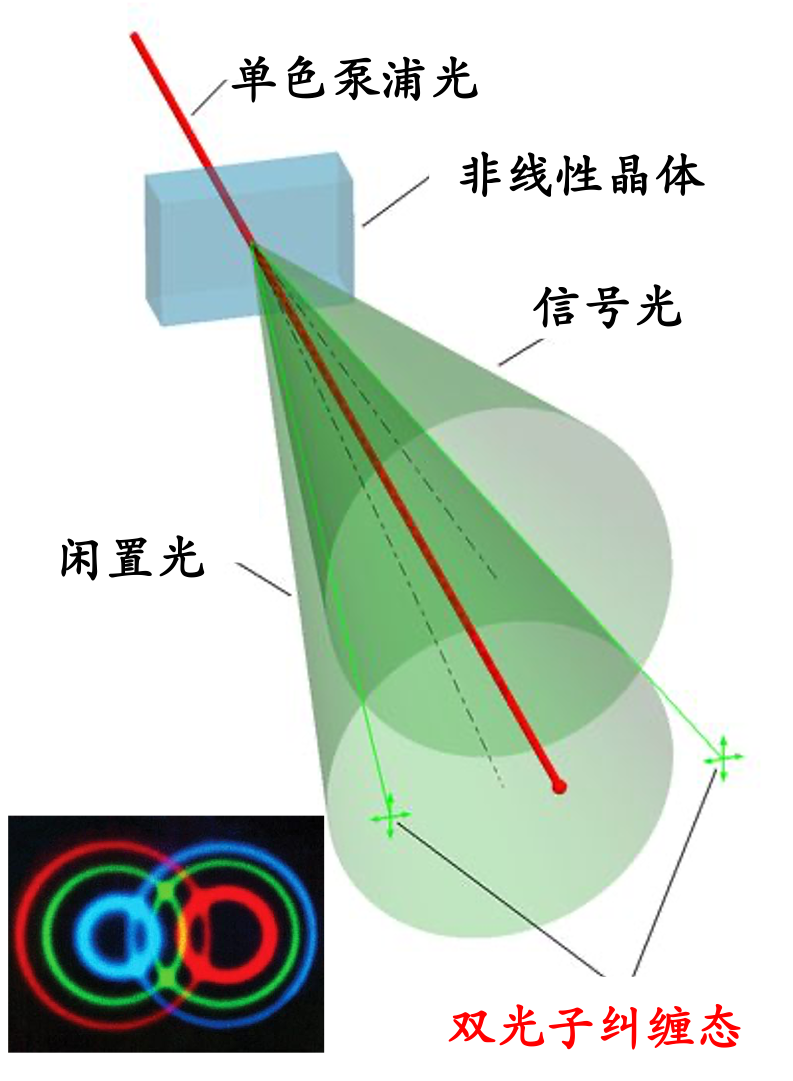
\includegraphics[width=0.3\textwidth]{figs/32.png}
    \end{center} 
    应用:
 \begin{enumerate}
     \item 单光子源 : 测得闲置光子,则必有信号光子! 由于产生光子对的概率很低, 同一时刻产生两个信号光子的概率趋零.  
     \item 纠缠光子双: 闲置光子与信号光子同时产生, 存在多个自由度的纠缠
 \end{enumerate} 
\end{frame}


\section{5. 压缩态的探测}

\begin{frame}
    \frametitle{平衡零差探测}
           \begin{center}
                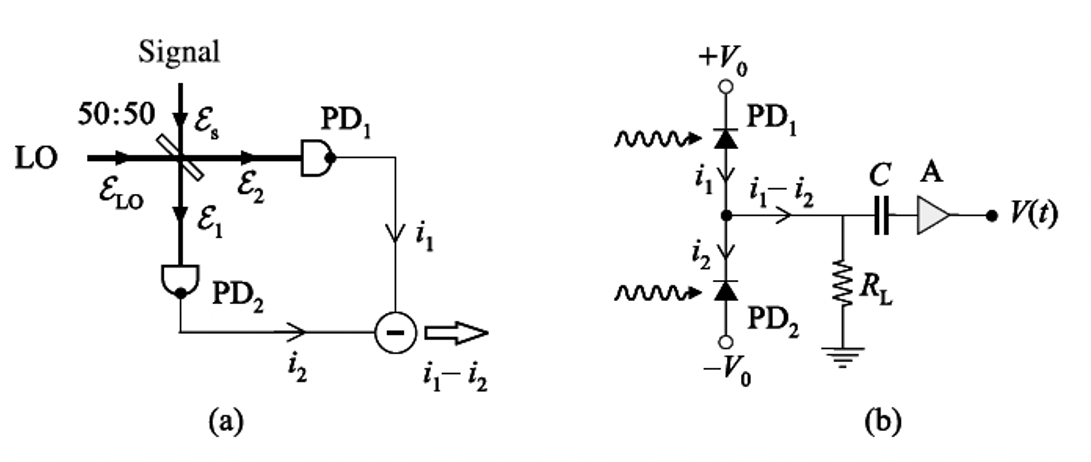
\includegraphics[width=0.8\textwidth]{figs/14.png}
           \end{center}
       基于一个平衡分束器(50:50)和两个光电二极管(PD)的平衡零差探测器实验装置图. ~~  
       LO: 本地振荡器, A: 放大器. 本地振荡器发出探测光场, 把信号光场(Signal)的信息带入输出电压V(t)中,从而实现对信号光场的探测.  
   \end{frame}
   
   
   \begin{frame}
       \frametitle{~}
       {\Bullet}信号分析: {\vspace*{0.3em}}
       零差意指两光场同频(中心频率~$\omega$~), 因此, 这是两光场相干问题. \\ 探测光场是强场 (经典处理) , 信号光场是弱场(量子化), 设两光场的相位差为$\phi$, 
       \[ E_L e^{i\phi} = E_L(\cos\phi + \sin\phi)\]
       \[ E_s  =  E_s ^{X_1}  + i E_s ^{X_2}\]
       注意到半波损失,输入输出关系为:
       \[ E_1  =  \frac{1}{\sqrt{2}} (E_L e^{i\phi} + E_s) = \frac{1}{\sqrt{2}} [ (E_L\cos\phi + E_s ^{X_1} ) + i (E_L\sin\phi + E_s ^{X_2} ) ]\]
       \[ E_2  =  \frac{1}{\sqrt{2}} (E_L e^{i\phi} - E_s) = \frac{1}{\sqrt{2}} [ (E_L\cos\phi - E_s ^{X_1} ) + i (E_L\sin\phi - E_s ^{X_2} ) ] \] 
      \end{frame}
   
      \begin{frame}
       \frametitle{}
       \[ \begin{aligned}
           V(t) &\propto  i_1 - i_2 \\ 
           &\propto  E_1 E^* _1 - E_2 E^* _2  \\ 
           &= 2 E_L ( \cos \phi E_s ^{X_1} + \sin \phi E_s ^{X_2} )
       \end{aligned} \]
       增加移相器\\  
       (1)  $\phi= 0, \pi, 2\pi, \cdots $, 可测得信号光场的$X_1$
       \[ V_1 \propto 2 E_L E_s ^{X_1} \]
       (2)  $\phi= \frac{\pi}{2}, \frac{3\pi}{2}, \cdots $, 可测得信号光场的$X_2$
       \[ V_2 \propto 2 E_L E_s ^{X_2} \]
       因此, 平衡零差探测可用来测量压缩态
      \end{frame}
   
      \begin{frame}
       \frametitle{}
       {\Bullet}噪声分析: \\ 
       如果没有信号光场的输入, 则相当于是真空场的输入, 噪声正是与探测光场同频的真空态的正交分量. 称为散粒噪声(shot-noise)  
   \end{frame}
   
   \begin{frame}
         \frametitle{}
         ~~\\ 
       {\Bullet}压缩真空态测量 \\ 
       如果是真空态被压缩, 则  $ V_1 \not= V_2$, 因此, 平衡零差探测可用来测量压缩真空态
         \begin{center}
              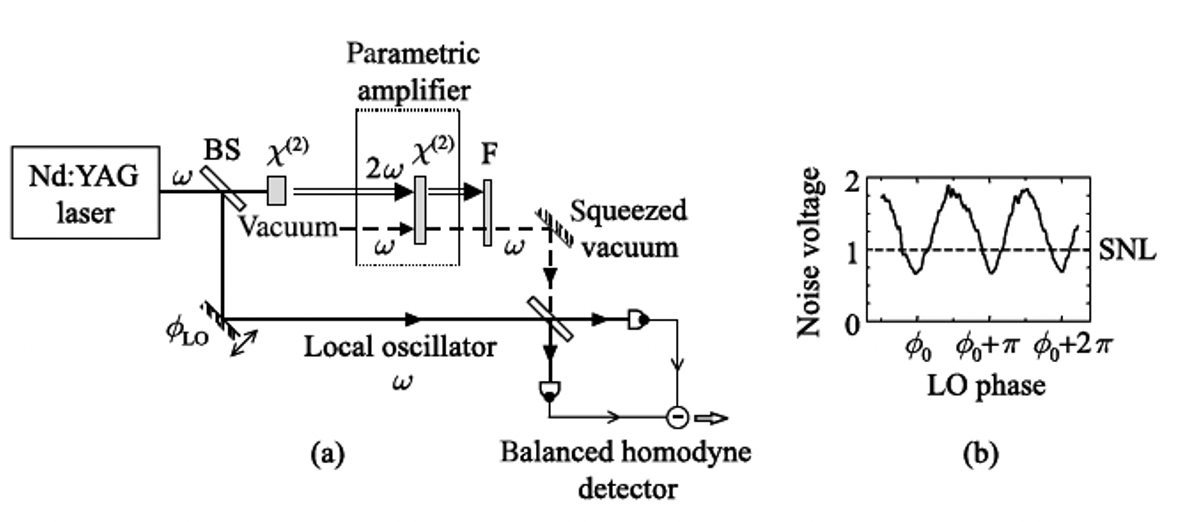
\includegraphics[width=0.9\textwidth]{figs/15.png}
         \end{center}
      \end{frame}